Let 
\begin{align}
X_{i}\in \{0,1,2, \ldots ,9\}
\end{align}
represent the digit at the $i^{th}$ place.

\begin{align}
\pr{X_i \notin \{0,5,9\}}=\frac{7}{10}=0.7     
\end{align}
If the k-digit number does not contain 0,5 or 9,
\begin{align}
\pr{X_{1} \notin \{0,5,9\} ,X_{2} \notin \{0,5,9\} ,\ldots, X_{k} \neq \{0,5,9\}  }
\end{align}
Since the events are independent, 
\begin{multline}\label{3:eq1}
  \pr{X_{1} \notin \{0,5,9\} ,X_{2} \notin \{0,5,9\} ,\ldots, X_{k} \neq \{0,5,9\}  }\\
  =  \pr{X_1 \notin \{0,5,9\}}\ldots\pr{X_k \notin \{0,5,9\}}
\end{multline}
\begin{align}
&=\prod_{i=1}^{k} 0.7\\
&=(0.7)^{k}
\end{align}

\begin{figure}[h!]
    \centering
    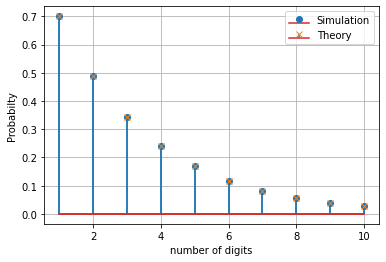
\includegraphics[width=\linewidth]{figs/3.png}
    \caption{Plot  }
    \label{3:}
\end{figure}